\begin{pages}
    \begin{Rightside}
    \selectlanguage{greek}
        \beginnumbering
		\pstart[
				\chapter{Τὸ σημεῖον τὸ πρῶτον}
				\markboth{The First Sign}
				]
		\renewcommand{\LettrineFontHook}{\PHtitl}
		\lettrine[lines=3]{Κ}{αὶ} τῇ ἡμέρᾳ τῇ τρίτῃ γάμος ἐγένετο ἐν Κανὰ τῆς Γαλιλαίας, καὶ ἦν ἡ μήτηρ τοῦ Ἰησοῦ ἐκεῖ· ἐκλήθη δὲ καὶ ὁ Ἰησοῦς καὶ οἱ μαθηταὶ αὐτοῦ εἰς τὸν γάμον. καὶ ὑστερήσαντος οἴνου λέγει ἡ μήτηρ τοῦ Ἰησοῦ πρὸς αὐτόν Οἶνον οὐκ ἔχουσιν. καὶ λέγει αὐτῇ ὁ Ἰησοῦς Τί ἐμοὶ καὶ σοί, γύναι; οὔπω ἥκει ἡ ὥρα μου. λέγει ἡ μήτηρ αὐτοῦ τοῖς διακόνοις Ὅ τι ἂν λέγῃ ὑμῖν, ποιήσατε. ἦσαν δὲ ἐκεῖ λίθιναι ὑδρίαι ἓξ κατὰ τὸν καθαρισμὸν τῶν Ἰουδαίων κείμεναι, χωροῦσαι ἀνὰ μετρητὰς δύο ἢ τρεῖς. λέγει αὐτοῖς ὁ Ἰησοῦς Γεμίσατε τὰς ὑδρίας ὕδατος. καὶ ἐγέμισαν αὐτὰς ἕως ἄνω. καὶ λέγει αὐτοῖς Ἀντλήσατε νῦν καὶ φέρετε τῷ ἀρχιτρικλίνῳ. οἱ δὲ ἤνεγκαν. ὡς δὲ ἐγεύσατο ὁ ἀρχιτρίκλινος τὸ ὕδωρ οἶνον γεγενημένον, καὶ οὐκ ᾔδει πόθεν ἐστίν, οἱ δὲ διάκονοι ᾔδεισαν οἱ ἠντληκότες τὸ ὕδωρ, φωνεῖ τὸν νυμφίον ὁ ἀρχιτρίκλινος καὶ λέγει αὐτῷ Πᾶς ἄνθρωπος πρῶτον τὸν καλὸν οἶνον τίθησιν, καὶ ὅταν μεθυσθῶσιν τὸν ἐλάσσω· σὺ τετήρηκας τὸν καλὸν οἶνον ἕως ἄρτι. Ταύτην ἐποίησεν ἀρχὴν τῶν σημείων ὁ Ἰησοῦς ἐν Κανὰ τῆς Γαλιλαίας καὶ ἐφανέρωσεν τὴν δόξαν αὐτοῦ, καὶ ἐπίστευσαν εἰς αὐτὸν οἱ μαθηταὶ αὐτοῦ.
		\pend
		\pstart
		Μετὰ τοῦτο κατέβη εἰς Καφαρναοὺμ αὐτὸς καὶ ἡ μήτηρ αὐτοῦ καὶ οἱ ἀδελφοὶ καὶ οἱ μαθηταὶ αὐτοῦ, καὶ ἐκεῖ ἔμειναν οὐ πολλὰς ἡμέρας. Καὶ ἐγγὺς ἦν τὸ πάσχα τῶν Ἰουδαίων, καὶ ἀνέβη εἰς Ἱεροσόλυμα ὁ Ἰησοῦς. καὶ εὗρεν ἐν τῷ ἱερῷ τοὺς πωλοῦντας βόας καὶ πρόβατα καὶ περιστερὰς καὶ τοὺς κερματιστὰς καθημένους, καὶ ποιήσας φραγέλλιον ἐκ σχοινίων πάντας ἐξέβαλεν ἐκ τοῦ ἱεροῦ τά τε πρόβατα καὶ τοὺς βόας, καὶ τῶν κολλυβιστῶν ἐξέχεεν τὰ κέρματα καὶ τὰς τραπέζας ἀνέτρεψεν, καὶ τοῖς τὰς περιστερὰς πωλοῦσιν εἶπεν Ἄρατε ταῦτα ἐντεῦθεν, μὴ ποιεῖτε τὸν οἶκον τοῦ Πατρός μου οἶκον ἐμπορίου. ἐμνήσθησαν οἱ μαθηταὶ αὐτοῦ ὅτι γεγραμμένον ἐστίν Ὁ ζῆλος τοῦ οἴκου σου καταφάγεταί με. 
		\pend
		\pstart
		ἀπεκρίθησαν οὖν οἱ Ἰουδαῖοι καὶ εἶπαν αὐτῷ Τί σημεῖον δεικνύεις ἡμῖν, ὅτι ταῦτα ποιεῖς; ἀπεκρίθη Ἰησοῦς καὶ εἶπεν αὐτοῖς Λύσατε τὸν ναὸν τοῦτον, καὶ ἐν τρισὶν ἡμέραις ἐγερῶ αὐτόν. εἶπαν οὖν οἱ Ἰουδαῖοι Τεσσεράκοντα καὶ ἓξ ἔτεσιν οἰκοδομήθη ὁ ναὸς οὗτος, καὶ σὺ ἐν τρισὶν ἡμέραις ἐγερεῖς αὐτόν; ἐκεῖνος δὲ ἔλεγεν περὶ τοῦ ναοῦ τοῦ σώματος αὐτοῦ. ὅτε οὖν ἠγέρθη ἐκ νεκρῶν, ἐμνήσθησαν οἱ μαθηταὶ αὐτοῦ ὅτι τοῦτο ἔλεγεν, καὶ ἐπίστευσαν τῇ γραφῇ καὶ τῷ λόγῳ ὃν εἶπεν ὁ Ἰησοῦς. Ὡς δὲ ἦν ἐν τοῖς Ἱεροσολύμοις ἐν τῷ πάσχα ἐν τῇ ἑορτῇ, πολλοὶ ἐπίστευσαν εἰς τὸ ὄνομα αὐτοῦ, θεωροῦντες αὐτοῦ τὰ σημεῖα ἃ ἐποίει· αὐτὸς δὲ Ἰησοῦς οὐκ ἐπίστευεν αὑτὸν αὐτοῖς διὰ τὸ αὐτὸν γινώσκειν πάντας, καὶ ὅτι οὐ χρείαν εἶχεν ἵνα τις μαρτυρήσῃ περὶ τοῦ ἀνθρώπου· αὐτὸς γὰρ ἐγίνωσκεν τί ἦν ἐν τῷ ἀνθρώπῳ.
		\pend
        \endnumbering
    \end{Rightside}
    \begin{Leftside}
        \beginnumbering
        \pstart[
        			\chapter{The First Sign}
        			]
        		\renewcommand\LettrineFontHook{\Zallmanfamily}
		\lettrine[lines=3]{A}{nd} on the third day there was a wedding in Cana of Galilee and Jesus’ mother was there; and even Jesus and his disciples were called into (invited to) the wedding. And being without wine (running out of wine, wanting wine), Jesus’ mother says to him, “They do not have any wine.” And Jesus says to her, “My dear woman, what do we have to do with this (lit. what to me and to you)? My time has not yet come.” And his mother says to the waiters, “Do whatever he tells you to do!” There were six water jars made out of stone — for the cleansing of the Jews — standing (around) and they were able to hold approximately two or three measures (80 - 120 litres) (of liquid) each. And Jesus tells them, “Fill the jars with water!”; and they filled them completely. And he tells them, “Draw out (some water) now and carry it to the master of the feast.” And they carried it over; and as the master of the feast tasted the water, it turned into wine and he did not know where it came from — the waiters carrying the water, however, knew. The master of the feast then calls the bridegroom and tells him, “Everyone (usually) drinks the good wine and — when they are (sufficiently) drunk — they then drink the lesser wine. You, however, have kept the good wine up until now.” This marked the beginning of the miracles which Jesus (did) in Cana of Galilee and revealed his glory; and his disciples believed in him. 
		\pend
		\pstart
		After this, Jesus, his mother, his brothers and his disciples went down to Capernaum and stayed there for a short time (lit. for not too many days). And the Jews’ feast of passover was near and (so) Jesus went up to Jerusalem; and he found in the (city’s) temple money changers and those which were selling cows (oxen), sheep and doves. And so, after making a whip out of a rope, he drove them all out of the temple — and the sheep and the oxen (as well). And he scattered the money changers’ coins and threw over their tables; and to those selling doves he said, “Take these things away from here; do not turn my Father’s house into a house of commerce!” And his disciples remembered that it is written that, “The zeal of your house consumes me (eats me up)”. 
		\pend
		\pstart
		The Jews, then, answered and said, “What sign are you showing us by doing this?” Jesus answered them and said, “Destroy this temple and within three days, I shall re-erect it!” And the Jews said, “This temple was in construction for forty-six years; and you will re-erect it in three days?” He, however, spoke of the temple of his body — so that when he rose from the dead, his disciples remembered that he said this and believed in both the scripture and the words which Jesus spoke.  And as he was in Jerusalem at the feast of the passover, many believed in his name (after) seeing the signs he did. But Jesus did not entrust himself to them; for he knows every (person) and did not need anyone to testify of mankind — for he knew what was within mankind. 
		\pend
        \endnumbering
    \end{Leftside}

\end{pages} 
\Pages

\clearpage
\thispagestyle{empty}
\null\vfill
\settowidth\longest{\huge\itshape […] and when I turned around I saw}
\begin{center}
\parbox{\longest}{%
  \raggedright{\huge\itshape%
    ``And as the master of the feast tasted the water, it turned into wine.'' \par\bigskip
  }
  \raggedleft\Large\MakeUppercase{Marriage at Cana — 1561, Tintoretto}\par%
}
\vfill\vfill
\clearpage\newpage
\end{center}
\newpage
\thispagestyle{empty}
\begin{center}
	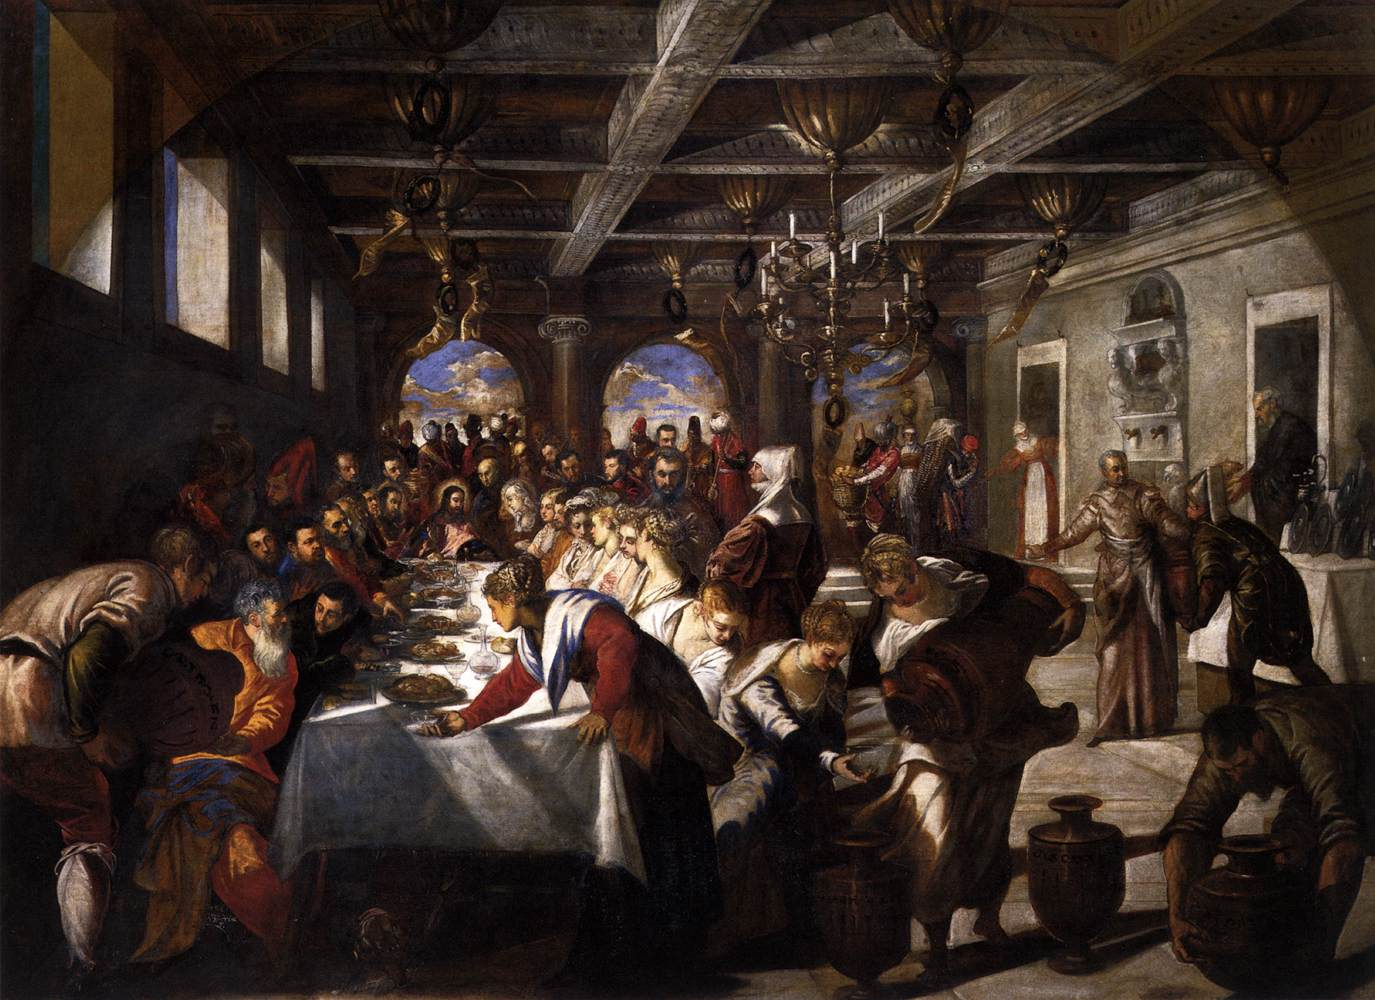
\includegraphics[angle=90, width=1\textwidth]{images/illustrations/tintorettomarriage.jpeg}
\end{center}
\vfill\vfill